\Problem
{گام سوم}
{
    \lr{size} 
    تصویر اصلی که 
    \lr{RGB} 
    است به صورت 
    \lr{1920x1080x3} 
    می‌باشد.
    
    با استفاده از دستور 
    \lr{rgb2gray} 
    آن را تبدیل به یک تصویر 
    \lr{grayscale} 
    با سایز 
    \lr{1920x1080} 
    می‌کنیم.
    
    در واقع تصویر اصلی دارای 3 کانال رنگی بوده است اما تصویر جدید دیگر عمق و کانال ندارد و هر پیکسل آن با 8 بیت یعنی عددی بین 0 تا 255 نمایش داده می‌شود. در صورتی که در دنیای 
    \lr{RGB} نیاز به 24 بیت داریم.
    
    عدد 0 معادل سیاه و عدد 255 معادل سفید است و مقادیر بین آن در واقع روشنایی بین این دو مقدار می‌باشند. فرمول تبدیل به صورت زیر است.
    
    \begin{center}
        $0.2989 \times R + 0.5870 \times G + 0.1140 \times B$
    \end{center}
    
    \begin{figure}[H]
        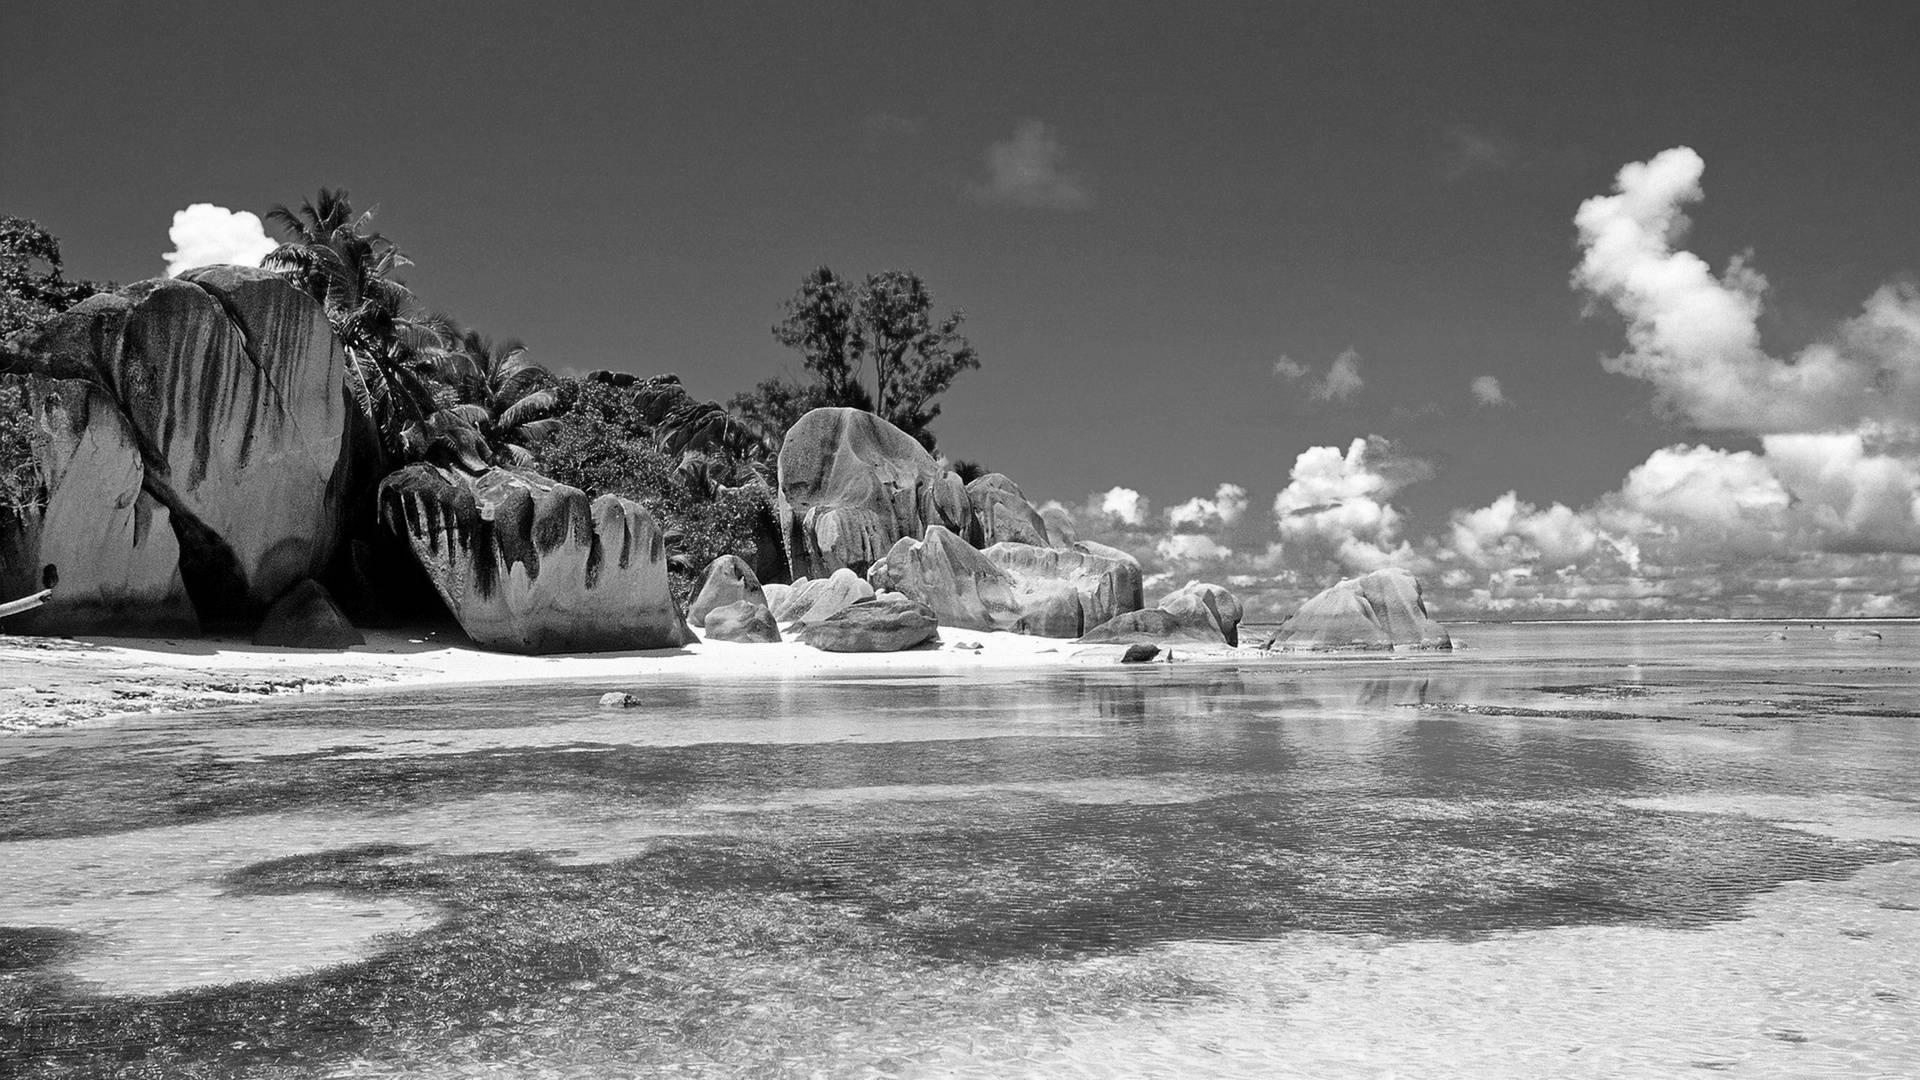
\includegraphics[width=15cm]{Images/Gray.jpg}
        \centering
        \caption{تصویر خاکستری}
    \end{figure}
    
    
}
